%\setcounter{chapter}{2}

\chapter{LHC and the CMS experiment}
\label{ch:cms}

\section{Introduction}\label{sec:cms_intro}
Large Hadron Collider (LHC) (see Fig. \ref{lhcmap}) is the most powerful particle accelerator that has ever been built. It is located at the border of the France and Switzerland, reutilising the tunnel used previously by the Large Electron Positron collider. The whole LHC story begins in 1977, when CERN director general Sir John Adams suggested that LEP tunnel can be reused to accommodate the future hadron collider of more than 3 TeV energies \ref{Sadenius}. At the 1984 ECFA-CERN workshop on a "Large Hadron Collider in the LEP Tunnel" \ref{LHC1984}, the plans for LHC were stated, where the primary ones were the BEH mechanism, Higgs boson, and the origin of masses of W and Z bosons. The parameters of the LHC machine were very ambitious: the centre-of-mass energy of 10 to 20 TeV, and a target luminosity of 10$^{33-34}\frac{1}{cm^{2}s}$. Luminosity is the coefficient which relates the cross section of the event under study to the number of events that will be generated in the LHC collision: $N_{events} = L \sigma_{event}$. Luminosity is the parameter control by the machine and for Gaussian beams \ref{Evans} can be written as:

$L=\frac{N^2_bn_bf_{rev}\gamma_r}{4\pi\varepsilon_n\beta^\star}F$

\noindent where $N_b$ is the number of particle in the colliding bunch, $n_b$ is the number of colliding bunches in the beam, $f_{rev}$ is the revolution frequency, $\gamma_r$ is the relativistic factor, $\varepsilon_n$ is the normalised transverse beam emittance, $\beta^\star$ is the beta function at the collision point, and $F$ is the factor related to the crossing angle at the interaction point (IP). The luminosity is not constant and decays with time due to the degradation of the initial circulating beams. Decay time is approximately 45 h, and 29 h to reach $1/e$ level. Adding contribution from the intrabeam scattering, scattering on the residual gas, etc, the final luminosity lifetime is about 15 h. 

Another useful variation of the luminosity parameter is an integrated luminosity. Integrating over the yield of a single run we get: 

 $L_{int} = L_0 \tau_L \left[  1- e^{\frac{-T_{run}}{\tau_L}}  \right]$, 

\noindent where $L_0$ is the initial luminosity, $T_L$ is the total length of the run, and $\tau_L$ is the luminosity lifetime. The optimum runtime thus is either 5.5 or 12 hours, which potentially leads to $80-120/fb$ of data with barn $b$ denoting a unit area of 10$^{28}$ $m^2$. 


\begin{figure}[H]
  \centering
  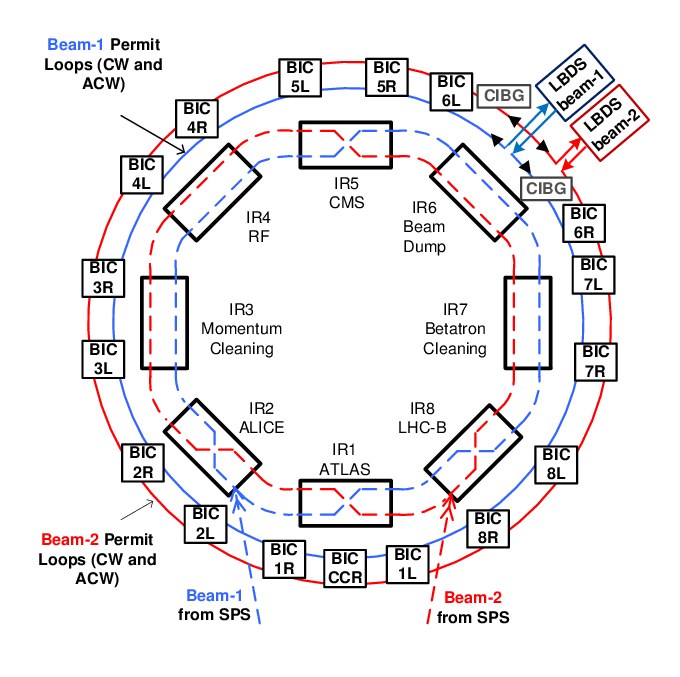
\includegraphics[width=0.75\textwidth]{LHC-beam-permit-loops}\\
  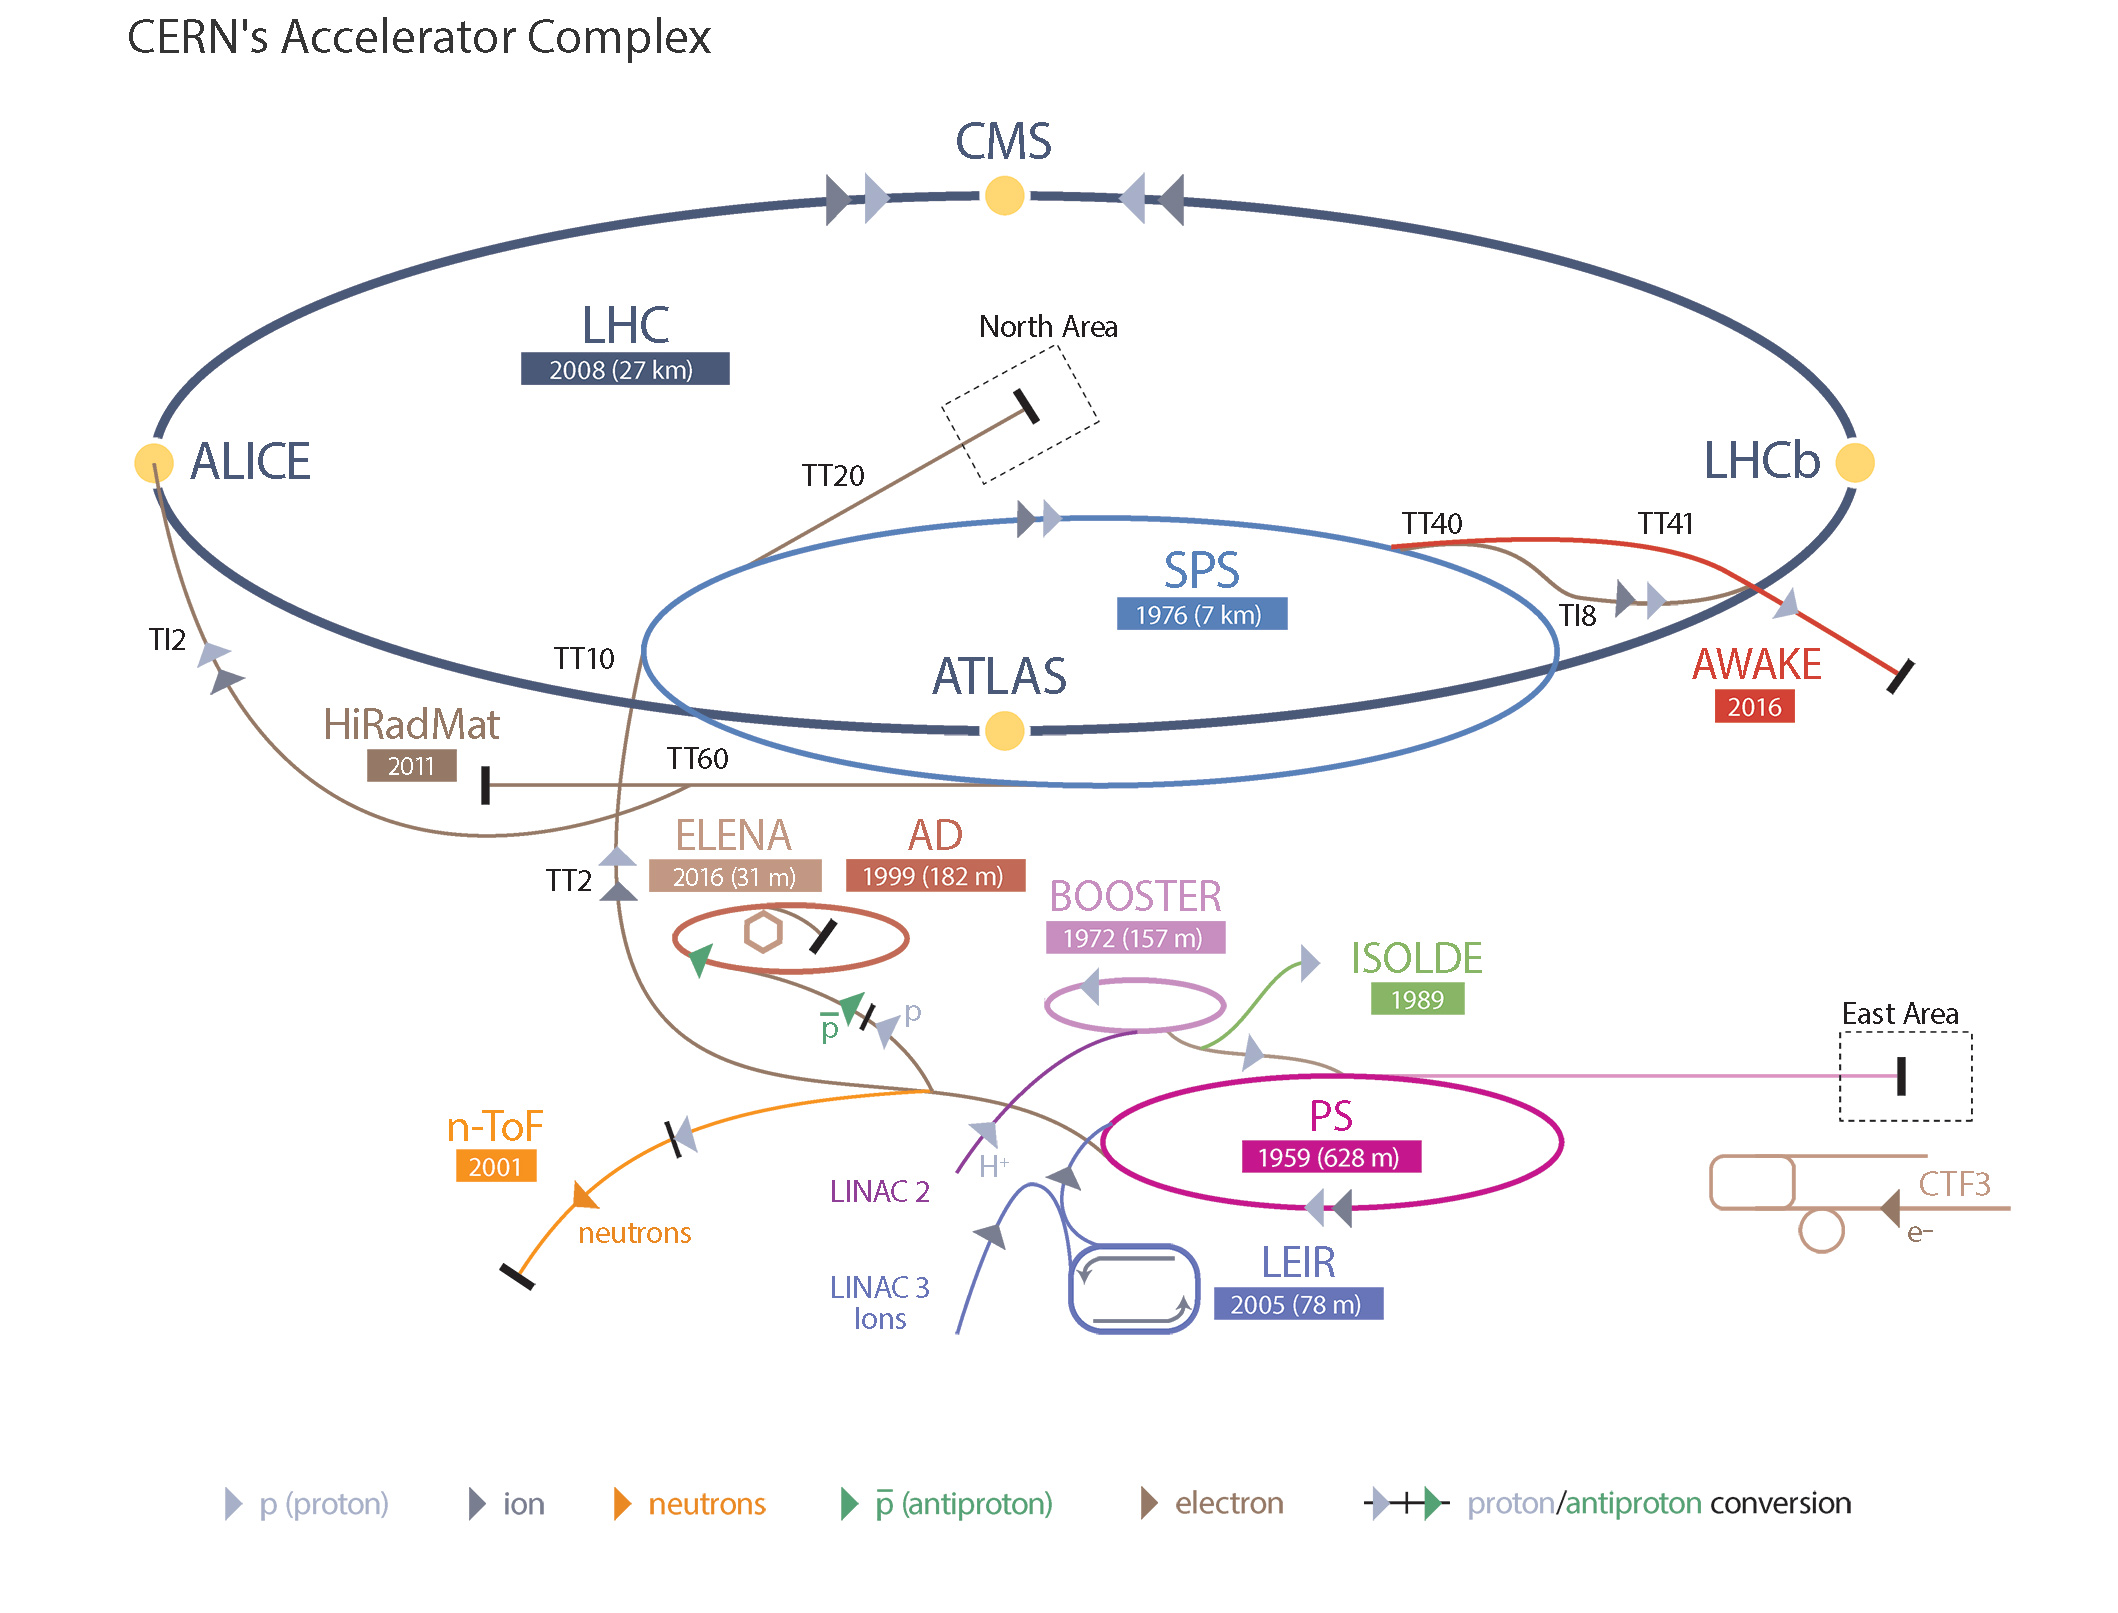
\includegraphics[width=0.75\textwidth]{LHC_default.jpg}
  \caption {Schematic layout of the LHC.}
  \label{lhcmap}
\end{figure}


\section{The LHC}\label{sec:lhc}
The first LHC budget plan was approved in 1996 and the final cost sum was completed in 2008. 4 years later the Higgs discovery happened, in 2012, quite fast for such a huge project! 
Now we will talk about the most important parts of the LHC complex one-by-one. Let us start with magnets. 

 
\subsection{The Magnets}\label{sec:magnets}
To keep the beam of protons on a circular orbit LHC needs strong magnets. The proven technology existed since Tevatron and relied on $NbTi$ superconductors. 1232 dipoles at 8 $T$, which are cooled to the below 2 $K$ temperature using superfluid Helium, bend the beam \ref{lhcDipole}. The dipole cold mass is in the so-called Helium bath and is cooled down to 1.9 $K$. Each of the 16.5 $m$ (with ancillaries) long and 570 $mm$ in diameter dipoles is slightly curved by 5.1 $mrad$ to help a chain of dipoles complete 360 degrees. The dipole is located inside of the dipole cryostat, which is a long cylindrical tube 914 $mm$ in diameter made of low-carbon steel. During the standard operation time the vessel contains the vacuum. 



\begin{figure}[H]
  \centering
  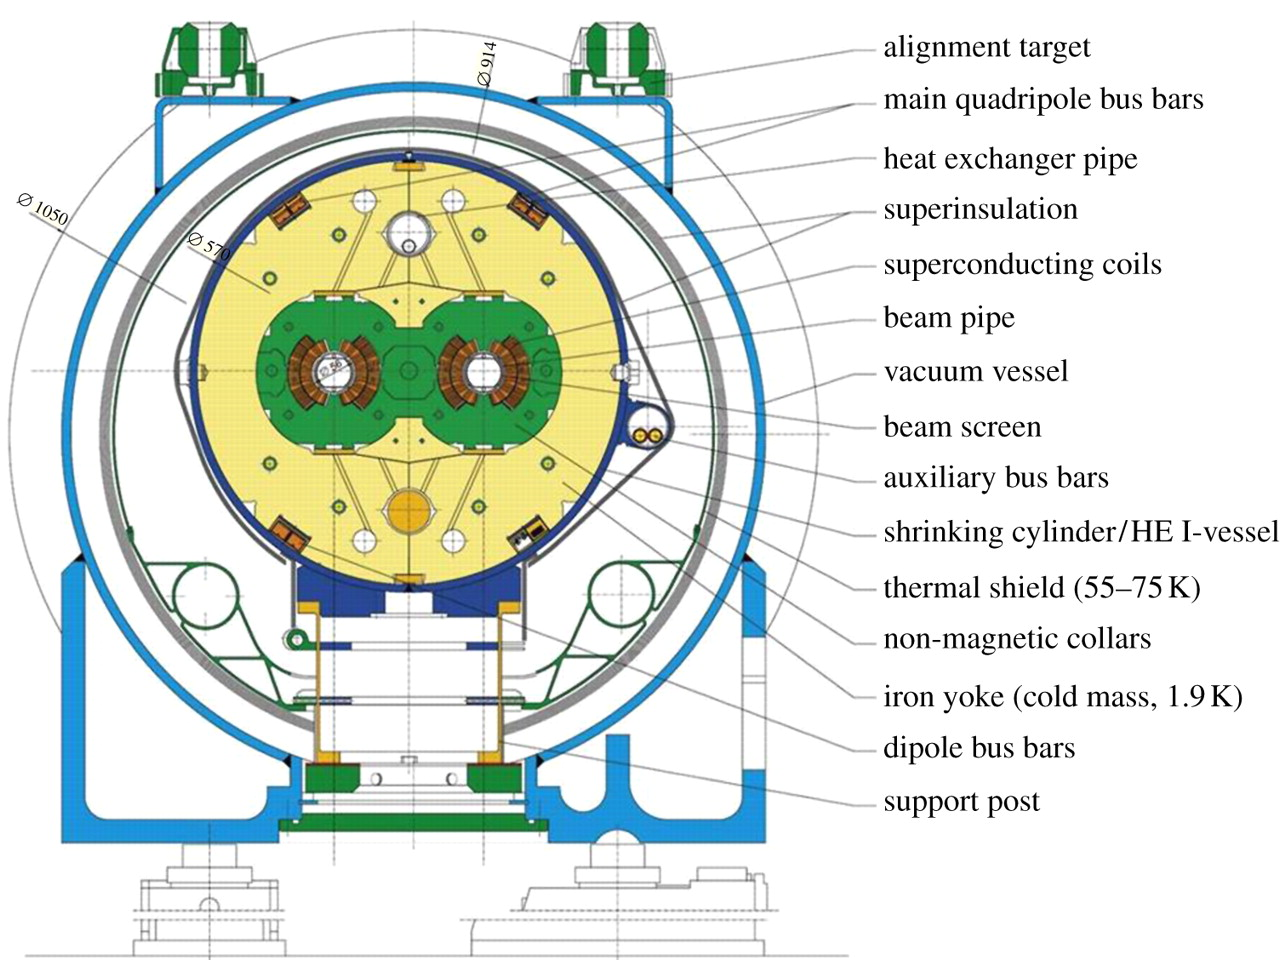
\includegraphics[width=0.9\textwidth]{lhcDipole}
  \caption[The cross section of the LHC dipole]{The cross section of the LHC dipole.}\label{lhcDipole}
\end{figure}


The material and the properties of the cables for the dipoles had to be carefully chosen. Each dipole coil is 56 $mm$ in diameter and is made of cables of two types. The cable in the inner layer contains 28 strands 1.065 $mm$ each. The outer layer contains 36 strands 0.825 $mm$ each \ref{cables}. 

To correct the orbit, higher order correctors are used with about 3800 single aperture and 1000 twin aperture magnets evenly spaces around the circular trajectory. 

Another important task that is performed with the use of magnets is the beam insertion, which is done at eight specific insertion locations. LHC also uses $NbTi$ magnets to accomplish this work. 


\begin{figure}[H]
  \centering
  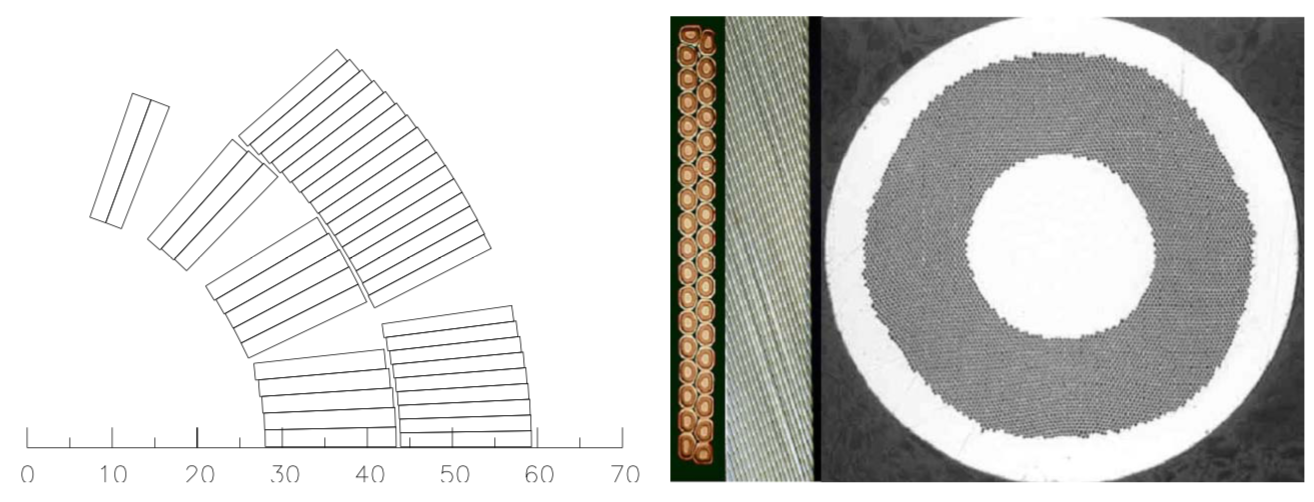
\includegraphics[width=0.9\textwidth]{cables}
  \caption[Cables of the dipole magnet]{Cables of the dipole magnet. Left: cross section view. Right: Strand and cables}\label{cables}
\end{figure}



\subsection{Radio Frequency System}\label{sec:rf}

The beam that comes from injectors will be placed, accelerated and kept on the orbit with the help of Radio Frequency (RF) cavities (see Fig. \ref{lhc_rfc}). The same system will be used to correct for injection errors in the beam direction. RF will be operating at the 400 $MHz$, which is 10 times more than the revolution frequency of 40 $MHz$. 

Four RF cavities grouped together into one cryomodule constitute an important accelerating module. If something happens to this module, it can be easily replaced in short period of time. 


\begin{figure}[H]
\centering
%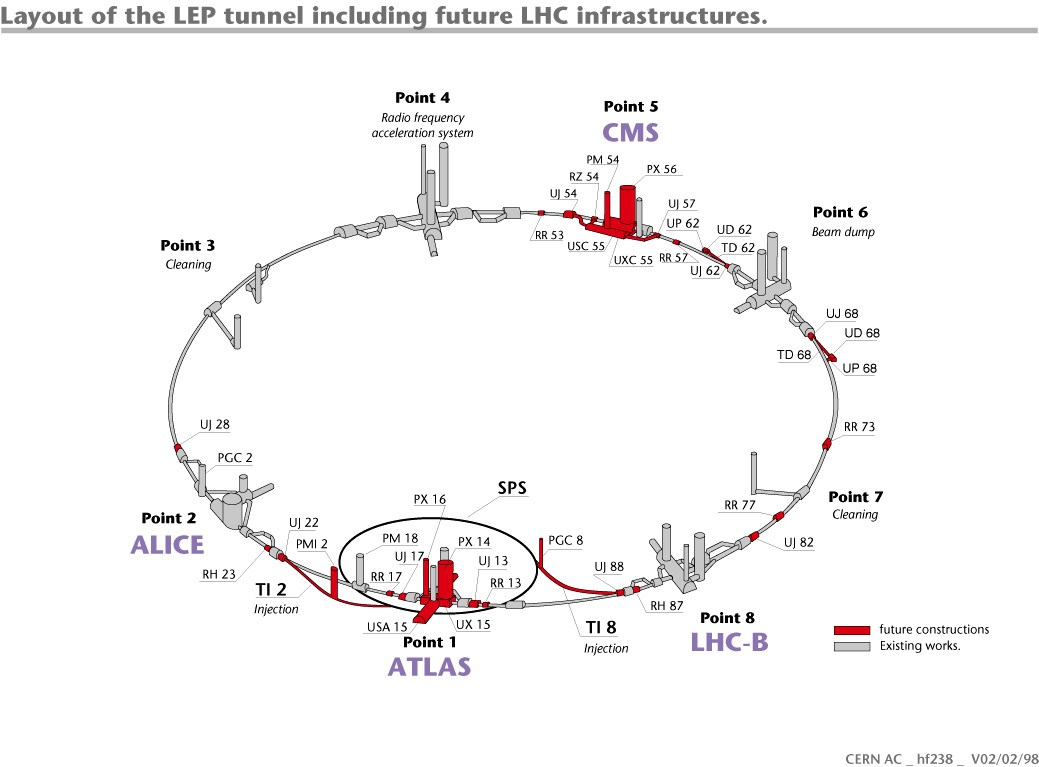
\includegraphics[scale=0.6]{lep}
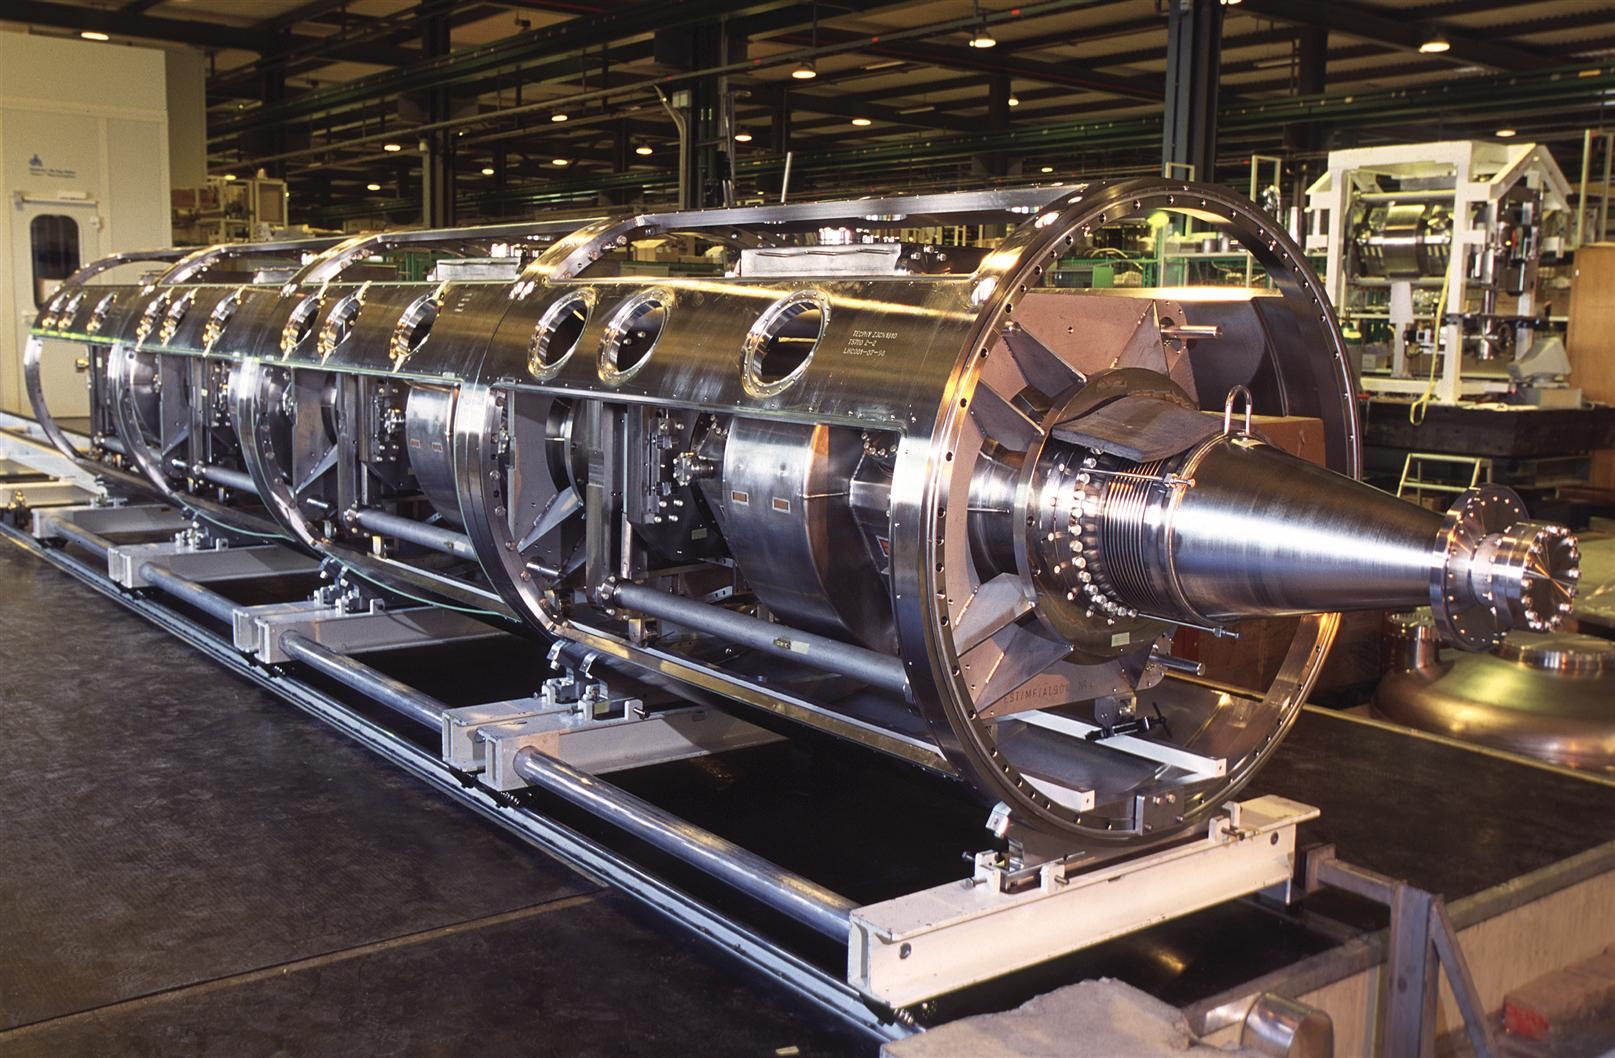
\includegraphics[width=7cm,height=4.2cm]{lhc_rfc}
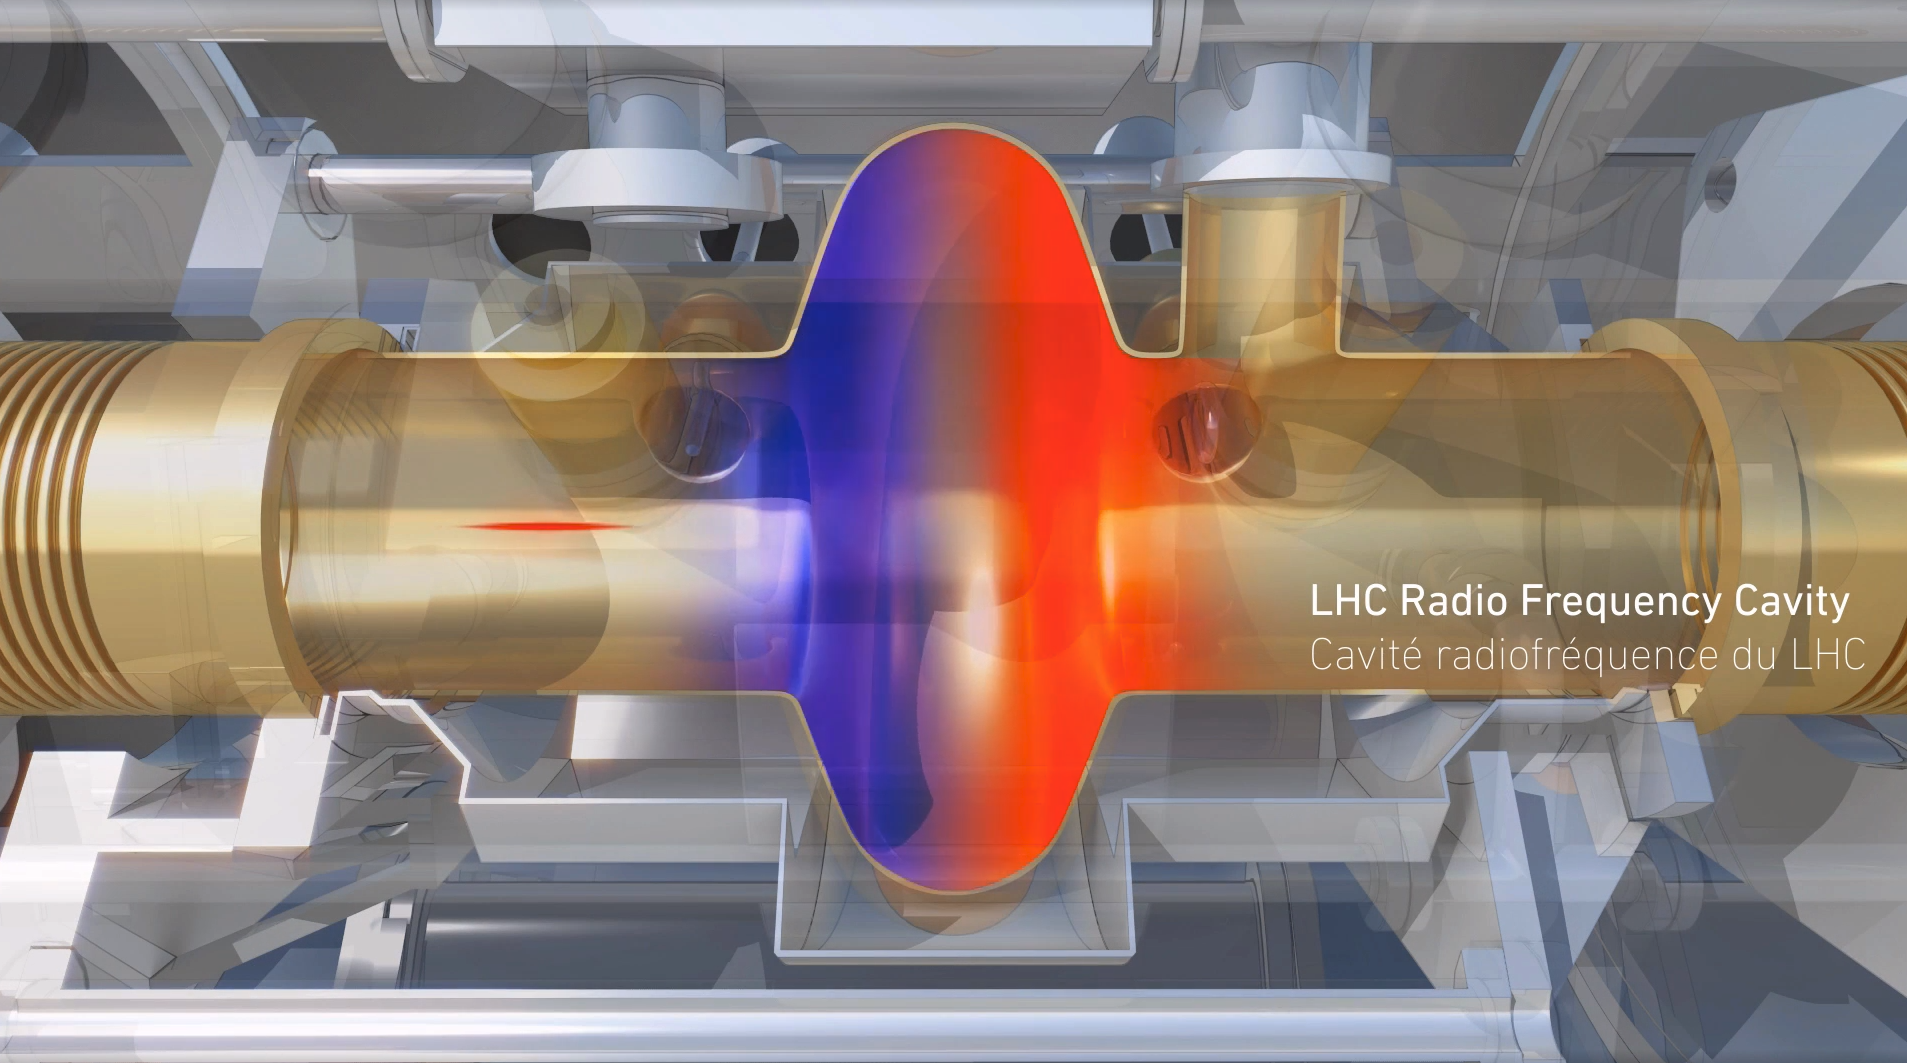
\includegraphics[scale=0.15]{rfc_lhc}
\caption[RF cavities module.]{LHC RF cavities. Left: a cryomodule with four RF cavities. Right: a single RF cavity schematic drawing. The colour field is used to highlight the fact of two field of the different polarity. }
\label{lhc_rfc}
\end{figure}


\subsection{Vacuum System}\label{sec:vacuum}


Three types of vacuum systems are necessary for the LHC proper operation. The vacuum system for the cryomagnets, the insulation vacuum for helium distribution, and, of course, the vacuum for the beam (VBS). As a convention, taking into account ionisation cross sections for gasses of the interests, cryogenic temperatures are expressed as corresponding gas densities normalised to the hydrogen. 
VBS, to ensure the 100 hours long run time, requires the equivalent hydrogen densities (EHD) to be below $10^{15} H_2 \frac{1}{m^3}$. To minimise the backgrounds from the experiments, the EHD at the interaction points should be $10^{13} H_2 \frac{1}{m^3}$. Those parts of the beam system, which operate under room temperatures, are under the pressure of $10^{-10}$ to $ 10^{-11}$ $ m$bar. All the vacuum section are subdivided into smaller modules to allow easy repair and fine tuning. 
VBS, as the most demanding in terms of the vacuum quality, have to be properly designed and must address a number of challenges, such as synchrotron radiation that significantly affects vacuum chambers in the arcs around the tunnel, as well as an electron cloud effect which exists along the length of the whole circle of the LHC. After the beam is inserted and is stabilised, the final adjustment of the VBS is needed to guarantee the perfect performance.

To finish the discussion of the VBS, let us discuss which heat sources have the main effect on the vacuum of the beam that must exist at the 1.9 K. 

\begin{itemize}
\item Synchrotron radiation (0.2 $W/m$ per beam)
\item Energy loss by nuclear scattering (30 $mW/m$ per beam)
\item Image currents (0.2 $W/m$ per beam)
\item Electron cloud related effects (vary)
\end{itemize}

To obstruct the heat sources mentioned above, specific beam screens are developed (see Fig. \ref{beam_screen}). Screens have elliptical shape, so-called racetrack shape, which gives extra space for cooling while optimises the aperture. 
Finally, the lifetime of the vacuum is mostly determined by the interactions of the vacuum gas nuclei with the protons of the beam. Values of the cross sections of such processes are given in \ref{Eggert:260711, Gr�bner:356437}.


\begin{figure}[H]
  \centering
  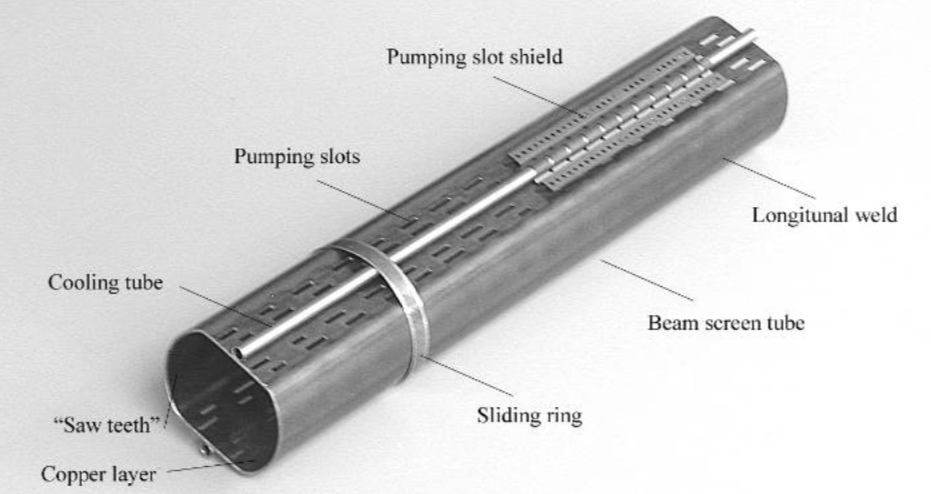
\includegraphics[width=0.7\textwidth]{beam_screen}
  \caption{Beam screen.}\label{beam_screen}
\end{figure}

\subsection{Powering}\label{sec:power}
To power the LHC, 1612 electrical circuits of 131 types are used. The magnets are powered in eight symmetrical sections. Some sections rely on all 131 types of circuits, while others may use only specific ones. To power the main quadrupoles which focus the beam, the power converters are located in the underground area. 
A total of 3286 current leads is needed to connect all the circuits and power cables. 1070 of the leads operate between 600 A and 13 kA (see Fig. \ref{13kA_lead}). The other leads work in the range 60 to 120 A. 

\begin{figure}[H]
  \centering
  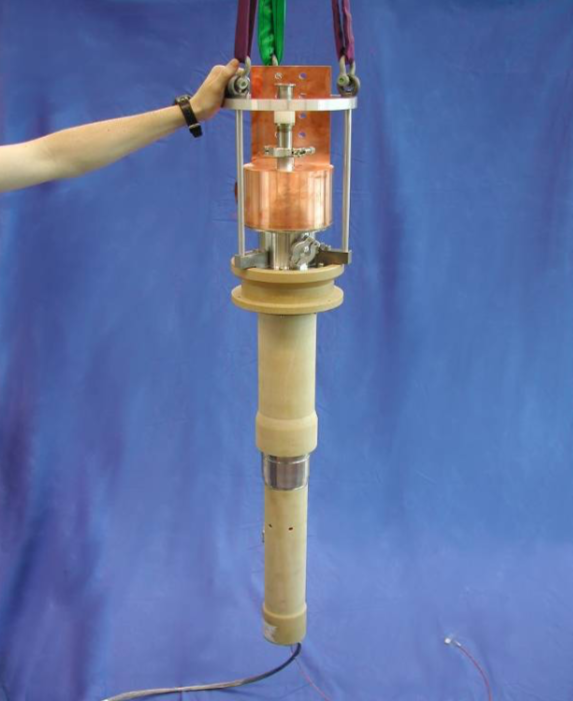
\includegraphics[width=0.7\textwidth]{13kA_lead}
  \caption{13 kA high-temperature superconducting current lead.}\label{13kA_lead}
\end{figure}


\subsection{Cryogenic system}\label{sec:cryogenic}
The cryogenic system (see Fig. \ref{cryo}) must supply the LHC cold mass of 37 Mkg within 15 days with the necessary temperature settings and work with the temperatures different by 75 K. The system must also be able to deal with the fast pressure raises and flow surges, and should be able to recover in a short period of time from such perturbations not to affect the run of the whole LHC. Another important point during the cryogenic design that had to be addressed is the fact that the LHC tunnel is inclined in the horizontal plane by 1.41 $^\circ$. This equals to 120 m difference in the vertical location of two diametrically opposite points of the tunnel with respect to the surface level and results in the additional hydrostatic pressure that can affect the flow of the cryogen. To avoid any instability of the LHC work like this, the gas is transported in the super-heated-vapour state. 

\begin{figure}[H]
  \centering
  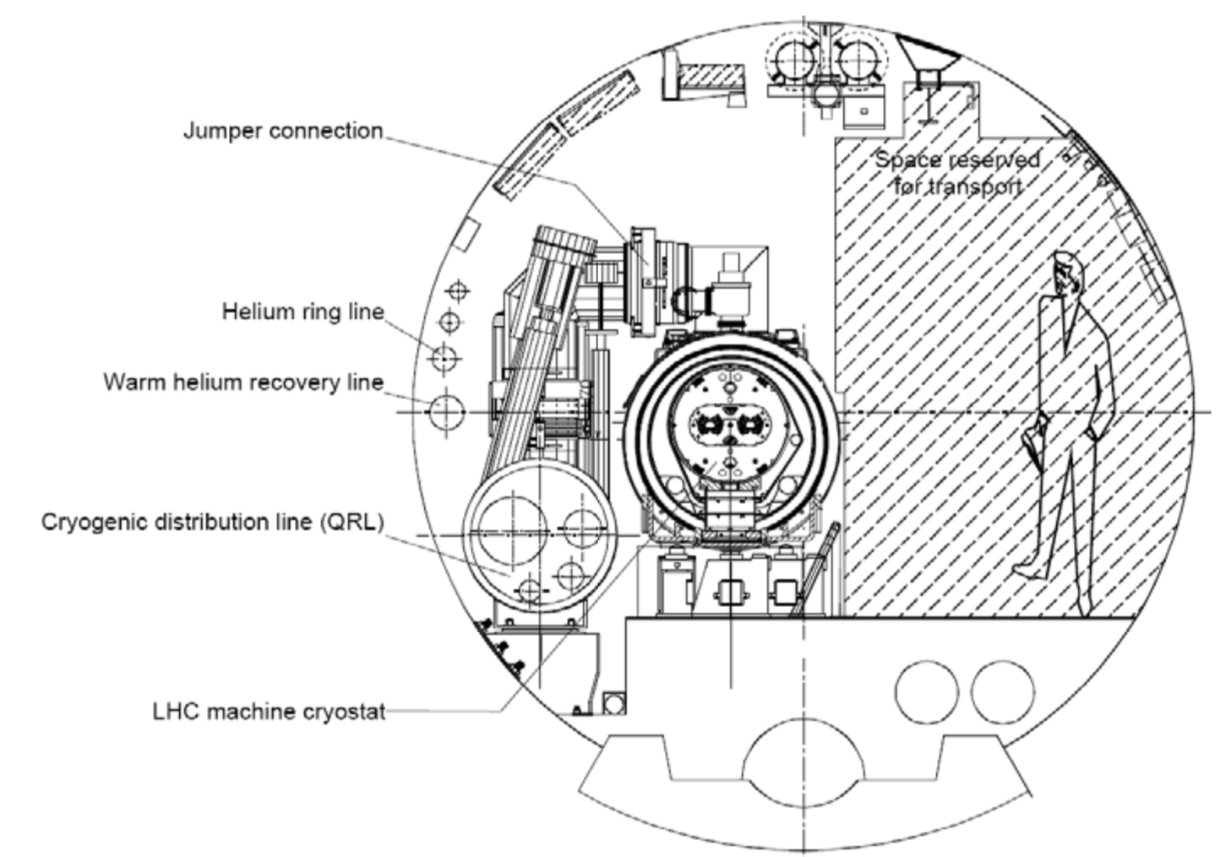
\includegraphics[width=0.7\textwidth]{cryo}
  \caption{Cross section of the LHC tunnel}\label{cryo}
\end{figure}


Since the cost of the production of 1.8 K temperature is high, several temperature levels are employed (see Fig. \ref{cryo_T_scale}):
 
\begin{itemize}
\item 50 to 75 K for the thermal shielding that protects the cold masses
\item 4.6 to 20 K for lower temperature interception and to cool the beam screens
\item 1.9 K for quasi-isotermal helium in the superfluid state to cool the magnet cold mass
\item 4 K for the transportation system that directs the 1.8 K helium from the exchanger to the 1.8 K refrigerator 
\item 4.5 K for RF cavities and lower sections of the high-temperature superconducting current leads
\item 20 to 300 K for upper sections of the high-temperature superconducting current leads
\end{itemize}

\begin{figure}[H]
  \centering
  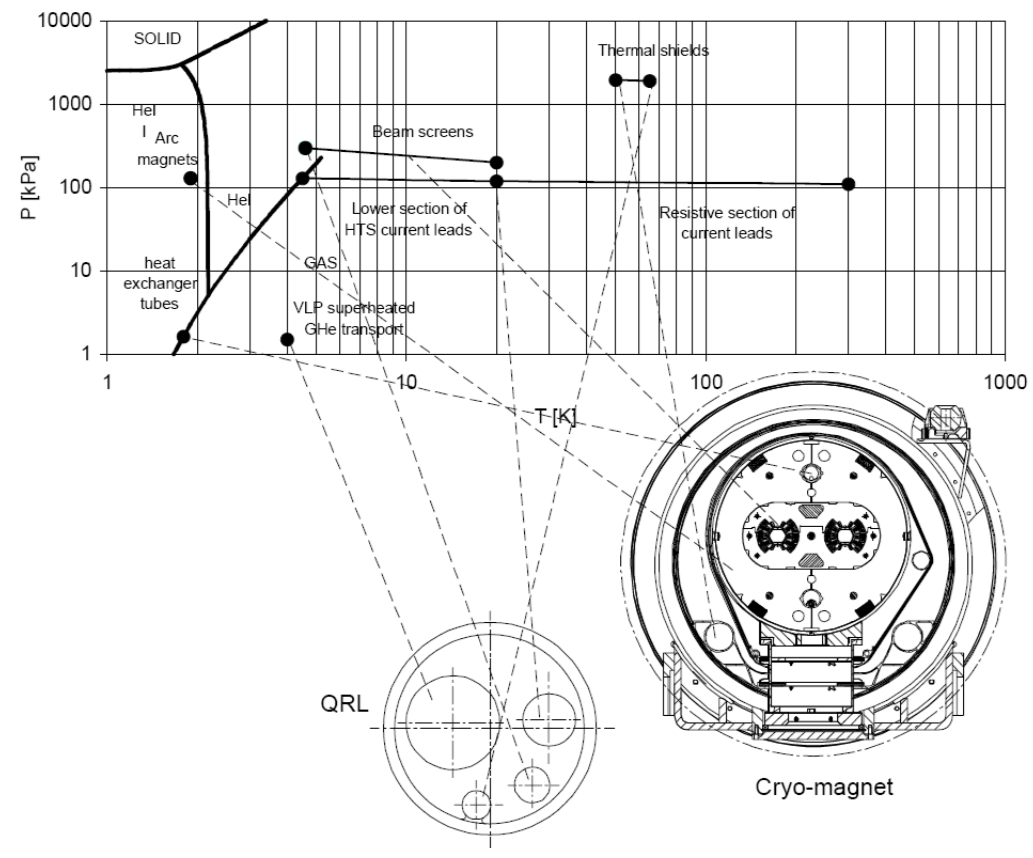
\includegraphics[width=0.7\textwidth]{cryo_T_scale}
  \caption{LHC cryogenic states and the temperature scale.}\label{cryo_T_scale}
\end{figure}


\subsection{Beam dumping system}\label{sec:dumping}

The LHC beam carries a lot of power and a well-designed and reliable beam extraction and dumping system is needed. Point 6 at LHC contains such system, which is able to fast-extract the beam in a loss-free way. The system for each ring comprises:

\begin{itemize}
\item 15 kicker magnets for extraction 
\item 15 steel septum magnets around the Point 6 interaction point
\item 10 modules of the dilution kicker magnets
\item the beam dump proper with the associated steel and concrete for shielding
\item dedicated dilution devices 
\end{itemize}

\subsection{Beam injection system}\label{sec:injection}
The injection at LHC is done at two points and for two beams separately: at Point 2 and Point 8. The beam comes to the insertion point from outside and below the machine level. A series of magnets and a kicker then deflects the beam horizontally and vertically to place the beam on the LHC orbit. To protect against the problematic injections and malfunctioning of the kickers, a series of the collimators correct the incoming beam. 

\subsection{LHC injection chain}\label{sec:injection_chain}

To place the beam at the final LHC orbit, the protons from the hydrogen bottle extracted from the hydrogen gas have to travel a long pass during which they are put into bunches and accelerated to the nominal collision speed. 

\begin{figure}[H]
  \centering
  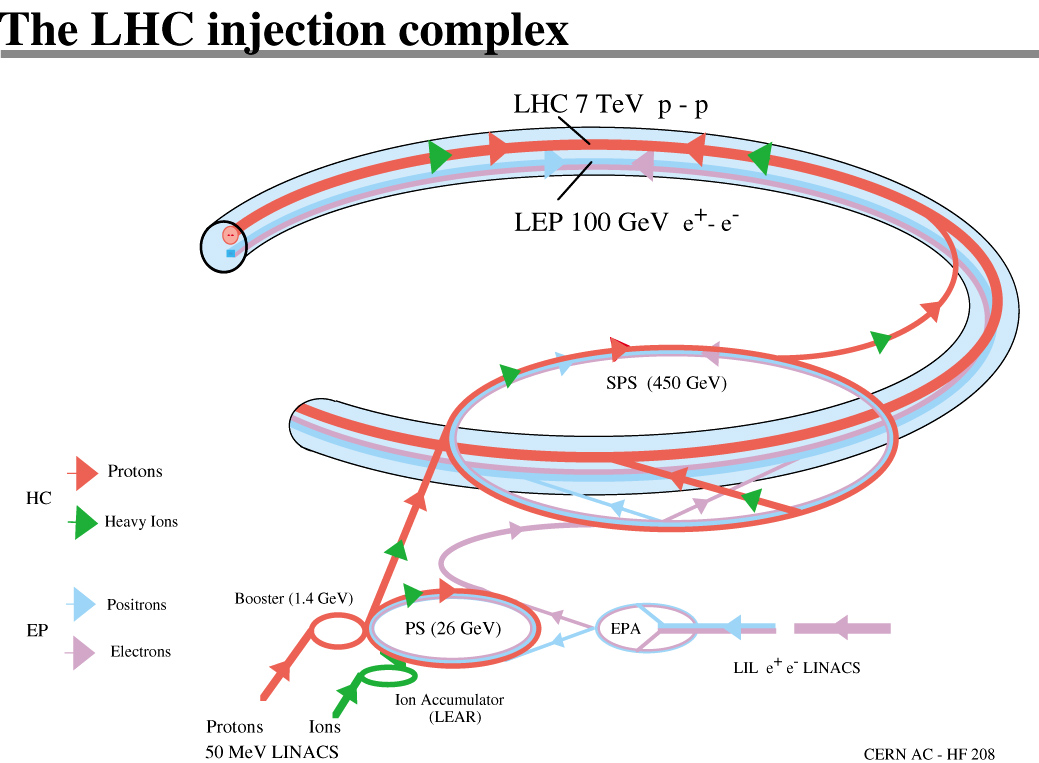
\includegraphics[width=0.7\textwidth]{lhc_complex}
  \caption{LHC injection complex.}\label{lhc_complex}
\end{figure}


The accelerator complex consists of: LINAC, Booster, Proton Synchrotron, Super Proton Synchrotron, and finally, the LHC main ring (see Fig. \ref{lhc_complex}). 

The whole LHC complex has to satisfy requirements of the final ring, such as:
\begin{itemize}
\item the beam emittance has to be compatible with the small aperture of the LHC superconducting magnets
\item the effect of the synchrotron radiation has to be taken into account when calculating the required cryogen needs for the intensity of the incoming beam
\item the beam-beam interactions that enhance the betatron oscillations
\item in the injector the space-charge limits have to be taken into account
\end{itemize}

\section{The CMS experiment}
The total inelastic cross section of the proton-proton interaction at $\sqrt{s}=14$ TeV will be about 100 $m$b. The detectors observe the event rate of nearly $10^{9}$ inelastic events per second. This flow of data is too large to be stored, and also, does not contain that many event of interest. Therefore, the trigger system must reduce the event rate to manageable 100 events per second. In addition, a pile up (PU) of 20-200 events overlaid with the event of interest will be expected, which results in about 1000 particles produced every 25 ns. All sub-detectors of CMS (see Fig. \ref{cms_cross_section}), thus, have to be able to work fast and in a good synchronisation with each other. 


\begin{figure}[H]
  \centering
  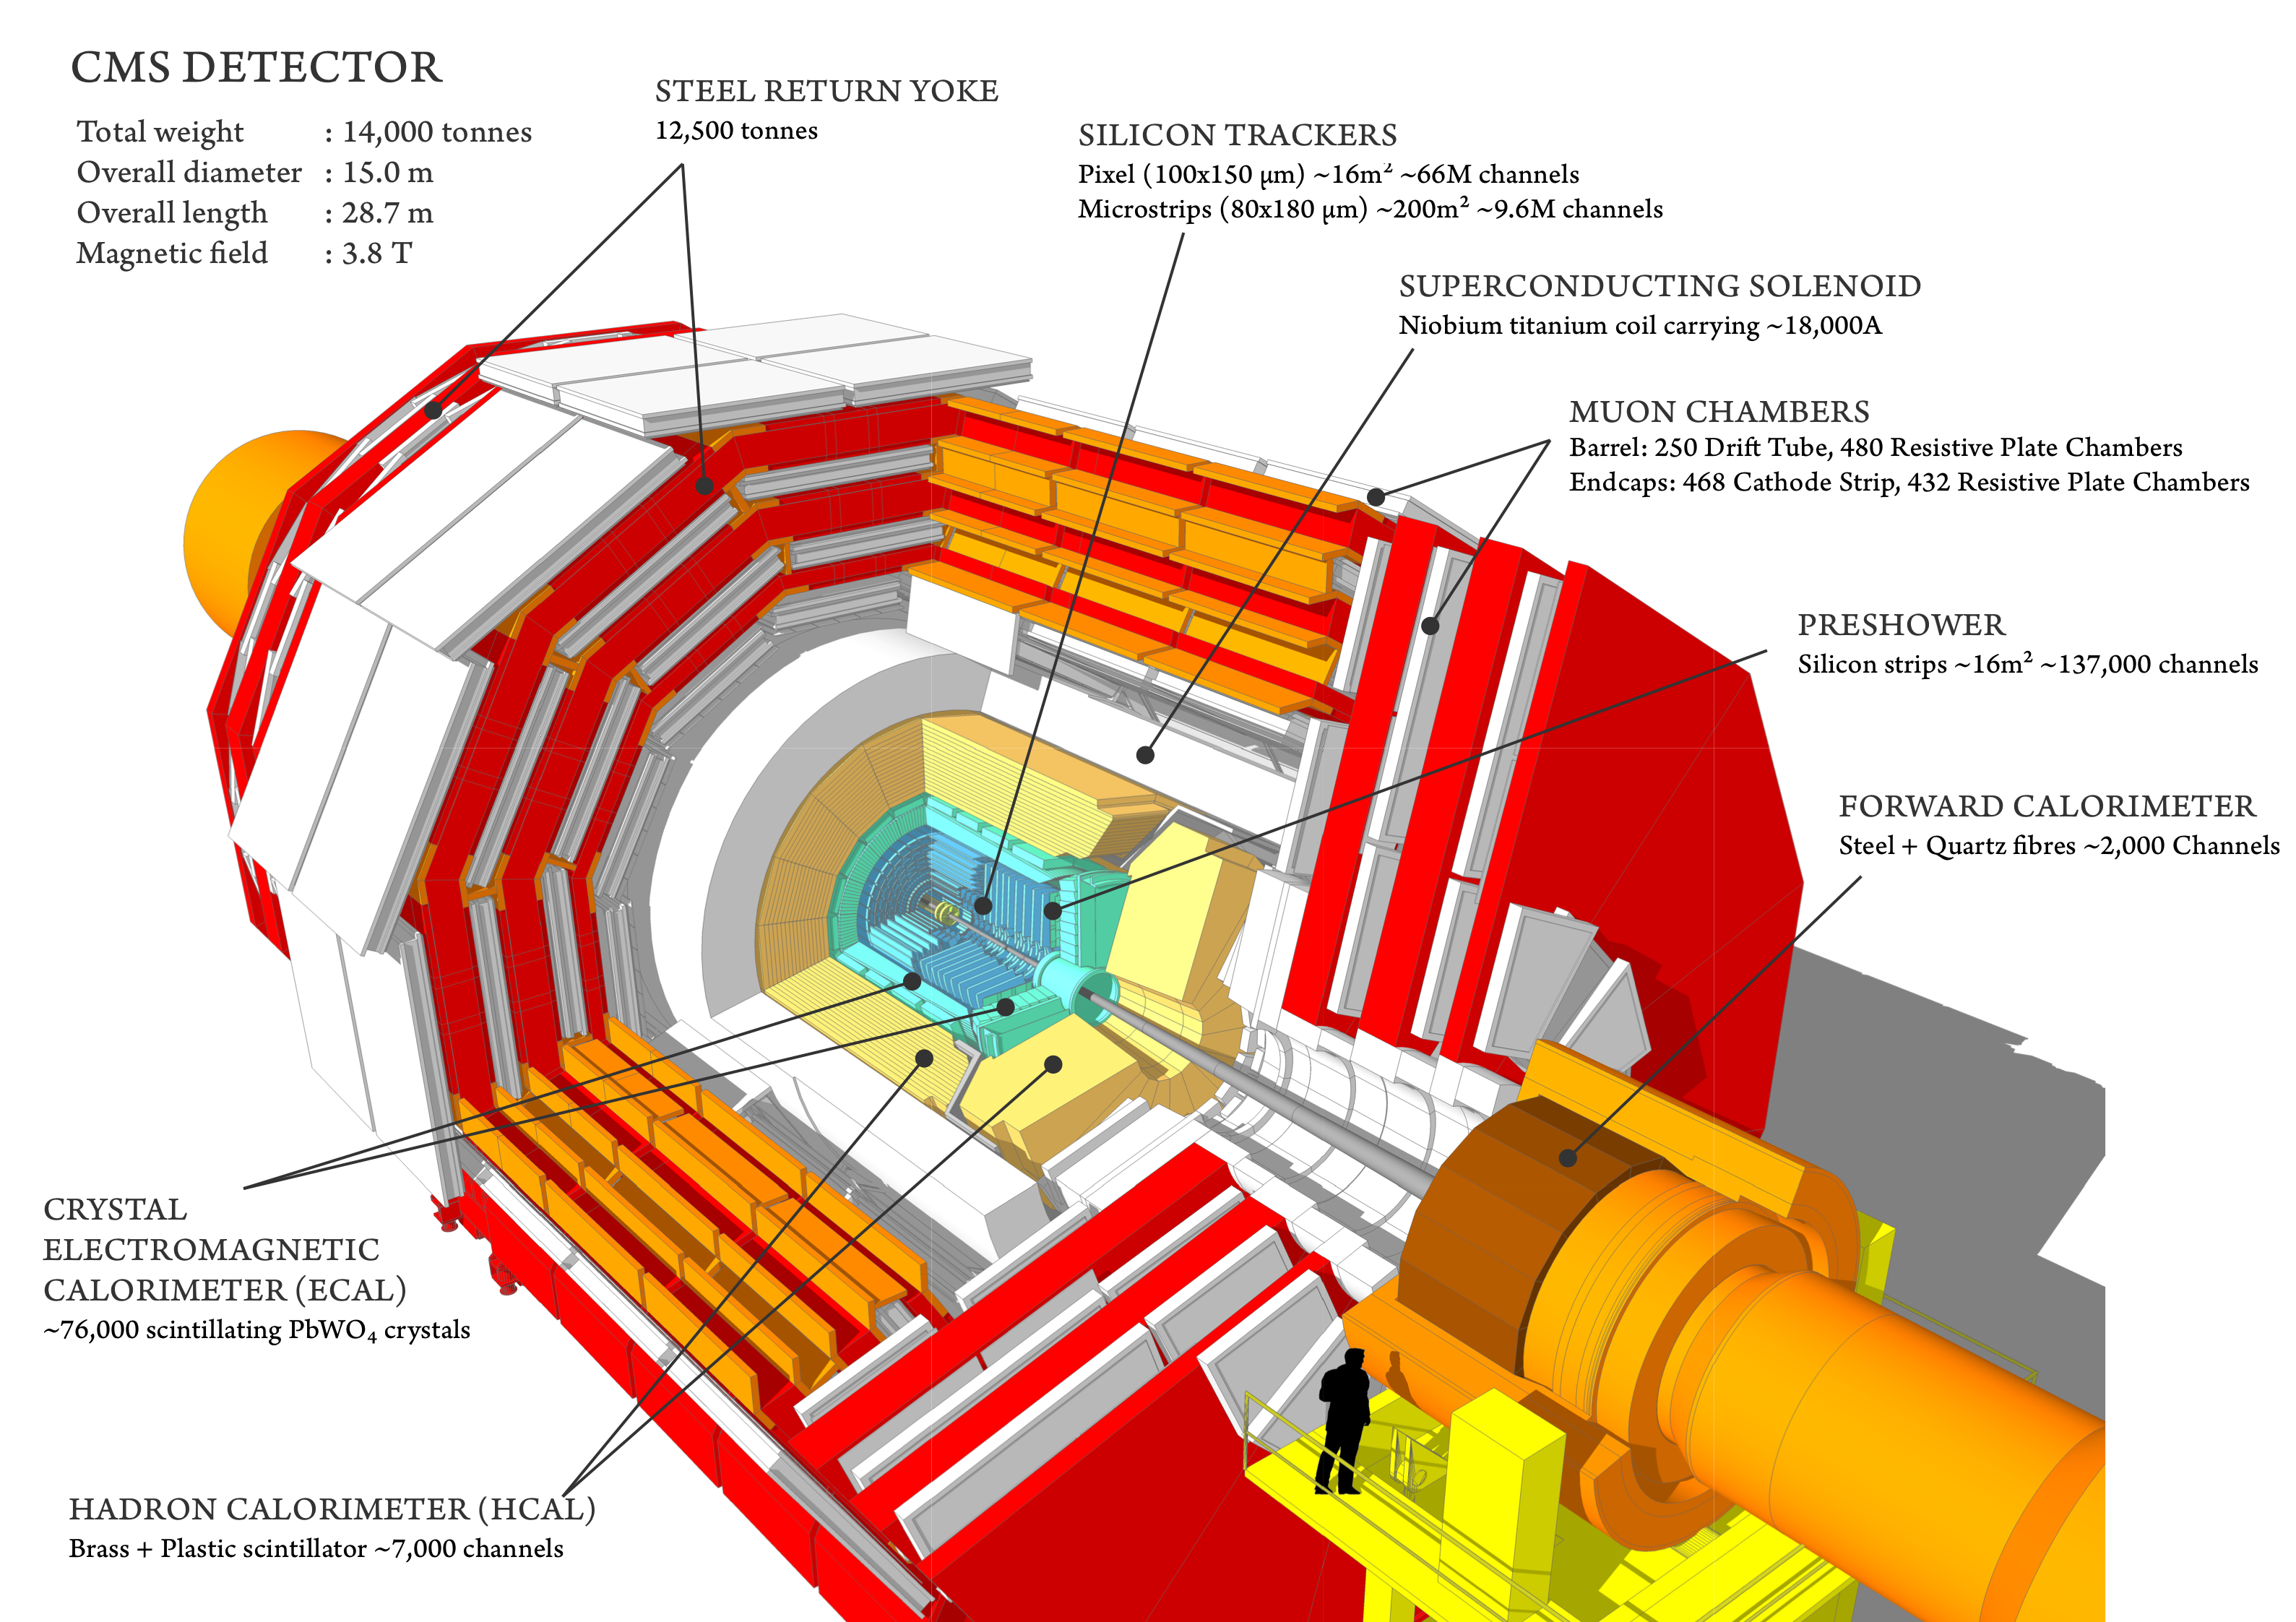
\includegraphics[width=0.9\textwidth]{cms_cross_section}
  \caption{CMS experiment with all sub-detectors shown.}\label{cms_cross_section}
\end{figure}

\subsection{The CMS challenging environment}
One can summarise all challenges and requirements that the CMS has faced in the following list:

\begin{itemize}
\item good muon momentum resolution over the momentum scale covering almost a TeV range, good dimuon resolution at the 100 GeV, and a capability to determine correctly the charge of the highly energetic muon all the way up to 1 TeV
\item good momentum resolution of the charged particles in the inner tracker. Emphasis on the efficient $\tau$ lepton and b-jets reconstruction
\item good performance of the electromagnetic calorimeter (ECAL), with the particular attention to the diphoton mass resolution, ability to reject efficiently $\pi^0$, ability to identify isolated photons and leptons
\item good missing transverse mass and dijet-mass resolution, which depends heavily on the performance of the hadronic calorimeter (HCAL)
\end{itemize}

The CMS design has been driven by the needs to have a large bending power, which is to be provided by the superconducting magnet, to be able to disentangle among each other various charged particles. The size of the magnet is 13 m in length and 6 m in inner diameter. 4 T solenoid provides 12 Tm bending power. The inner diameter is large enough to host the inner tracker and the ECAL. To address the high multiplicity problem, the CMS inner tracker uses 10 layers of the silicon microstrip detectors. The inner barrel contains four layers of strips and the outer barrel has six layers. Each silicon sensor is 320 $\mu m$ in height and a specifically designed overlay of strips provides a spatial resolution of 13-38 $\mu m$. About the same resolution is achieved by the other tracker. The whole tracker contains 15148 silicon modules with the 9.3 million strips. Tracker provides the experiments with the tracks information left by the charged particles traversing its material. 

To further improve the impact parameter determination and secondary vertex reconstruction, three layers of the silicon pixel detector are inserted near the interaction region. Pixel detector is composed of 1440 silicon pixel detector modules organised in three concentric cylindrical layers, and also two disks in the forward regions. 


The ECAL technology is based on the on the lead tungstate crystals ($PbWO_4$). The ECAL measures the energy deposited by photons and electrons. ECAL contains 75848 crystals where the energy showers will be produced by the particles releasing their energy when interacting with the material of the crystals. Before the ECAL, a preshower system is placed to reject $\pi^0$. It contains layers of lead radiators followed by layers of the silicon strips to initiate and subsequently to measure the energy of the particle. The ECAL measured energy of the particles is a function of the stochastic term (S), noise (N), and a constant term (C). 

\begin{equation}
  \left(\frac{\sigma}{E}\right)^2 = \left(\frac{S}{\sqrt{E}}\right)^2 +
  \left(\frac{N}{E}\right)^2 + C^2
  \label{eq:ecal}
\end{equation}

The ECAL is surrounded by the HCAL system which is based on the brass/scintillator sampling hadronic technology. HCAL measures energy of particles made of quarks. Central part is later covered by the $\textit{tail-catcher}$ leaving 11 hadronic interaction lengths to the particle interactions.  
Further, the forward calorimeter is used to ensure the coverage in $\eta$ up to 5. Note, that the coverage of ECAL and HCAL are about up to $\eta=3$.  

Additional dedicated detectors such as  CASTOR, ZDC, etc, ensure that the detector has a full $4\pi$ coverage. HCAL does not fully absorb energy of the the particles traversing its medium, except very low energy particles, thus the energy of the particles is sampled to estimate the total amount.  

Overall, the CMS detector is 21.6 m in length and 14.6 m in diameter. The weight of the whole construction is near 12 500 tons. ECAL covers more than 25 radiation lengths, HCAL, from 7 to 11, depending on the $\eta$ region. Outer HCAL is located outside of the magnet.

The superconducting magnet of CMS provides the experiment with almost 4 T magnetic field and is operated at the 4.7 K temperature. 
Additionally, a magnet yoke is made of five barrel wheels is used for the magnetic flux return and serves as a support for the embedded muon system, which is located outside of the ECAL and HCAL systems. Muons are energetic enough to traverse the ECAL and leave the detector. Tracks in the muon system will be used to reconstruct standalone muons, and in combination with the tracker, to reconstruct the global muons.  


\subsection{CMS coordinate system}
It is useful to introduced a convenient coordinates system used by the CMS experiment. We will use rapidity and pseudorapidity many times in the analysis section of the thesis. The coordinate system employed by the CMS uses the rapidity, y, and pseudorapidity, $\eta$. They are derivatives of the log functions of the energy and a projection of the momentum on the z axis and the angle $\theta$ with respect to the beam axis (see Fig. \ref{coord} \ref{MonroyMontanez:2639240}):

\beqn
y=\frac{1}{2}ln\frac{E+p_z}{E-p_z} \qquad \eta=-ln \left(tan\frac{\theta}{2}\right)
\label{eqn:eta}
\eeqn


\begin{figure}[h!]
  \centering
  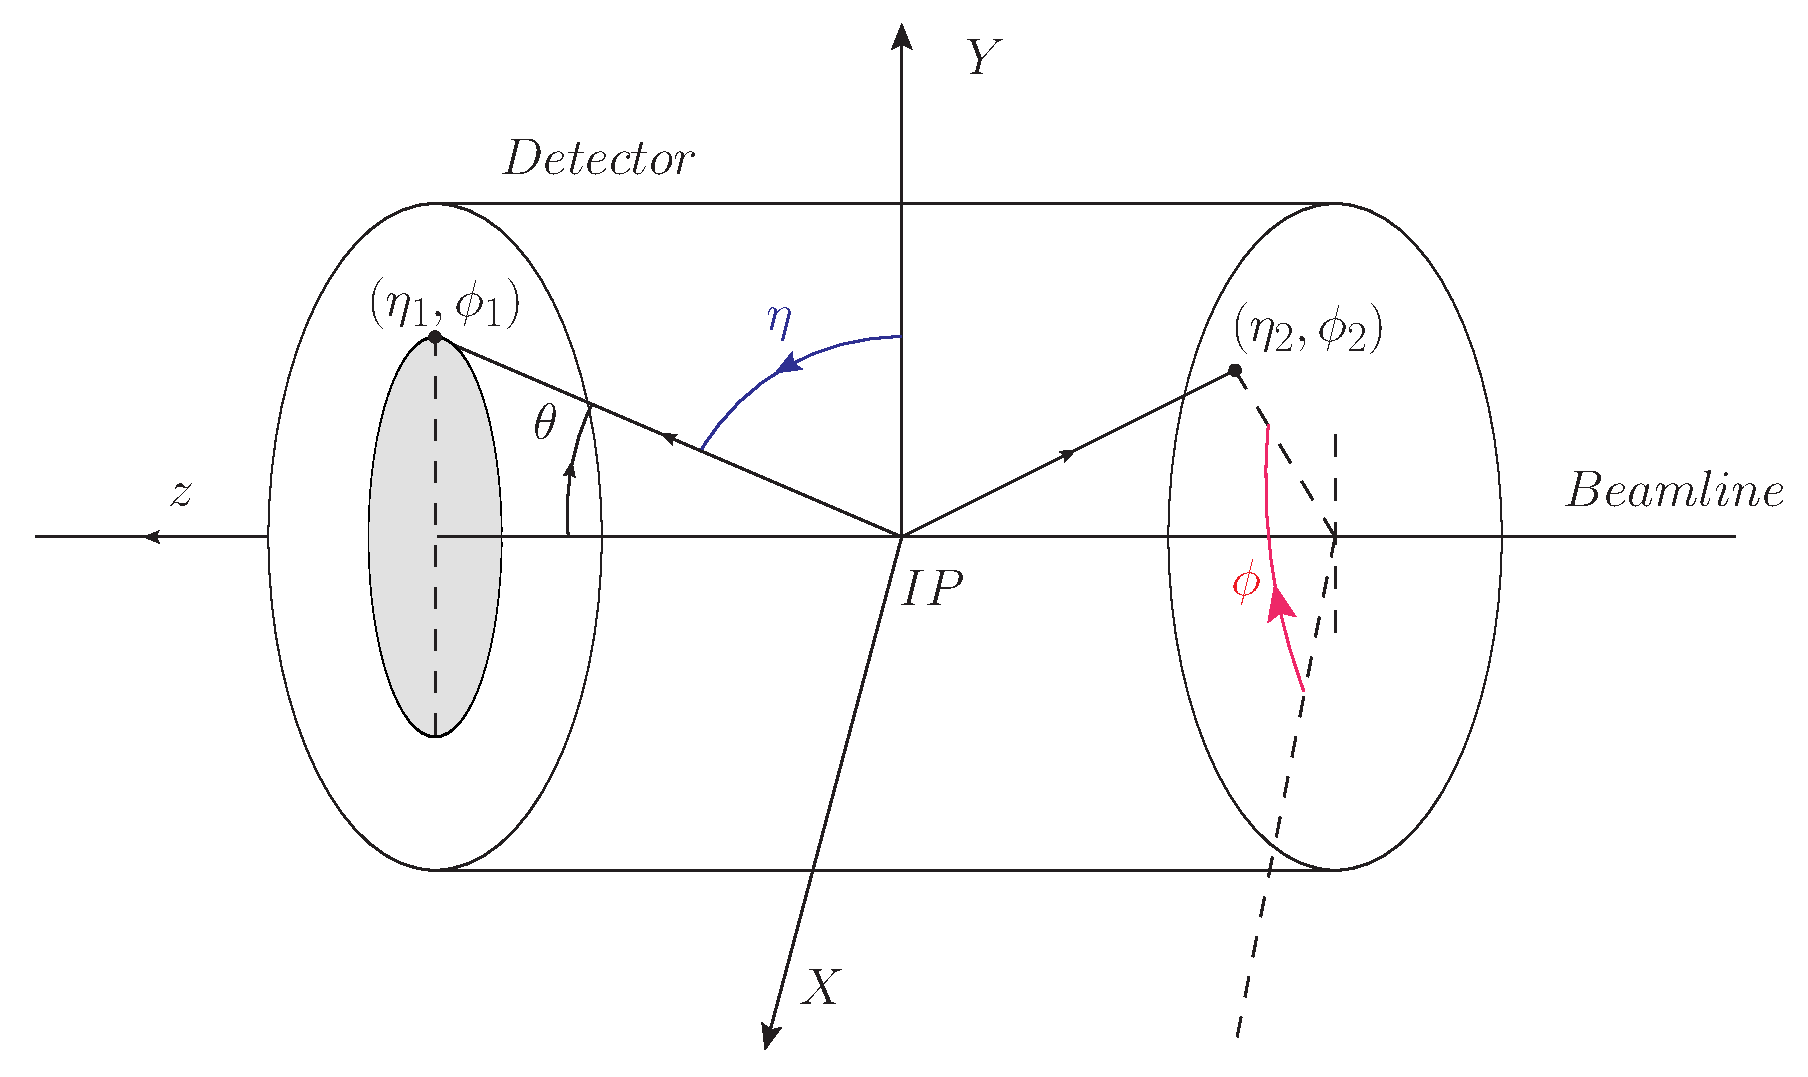
\includegraphics[scale=0.4]{coord}
  \caption[Coordinate system of the CMS detector]{Coordinate system of the CMS detector.}
  \label{coord}
\end{figure}

